%!TEX root = ../Masterthesis.tex
\chapter{System Evaluation}
\section{Camera hardware and control}
The image  processing of the camera frames on the raspberry can be a significant bottleneck for the system. Real time evaluation demands the processing time of a frame to be in the range of the time of the camera FPS. With the current system setup running at 30fps, this means that the image processing time, containing frame readout and downstream processing of the images, has to be done in about $1/30s$ or 33 ms to achieve "real time" processing. Professional stereoscopic setups use cameras with global shutters and a synchronization signal. This enables a sub frame synchronization of the two camera systems. The cameras used in the prototype setup use a rolling shutter instead. Since these cameras are designed to be of easy use for the normal consumer, they lack means of external synchronization. Furthermore, electrical drawings as well as controlling software are closed source. To achieve a from of hardware synchronization, a large amount of reverse engineering would be needed. The multi layered circuit board of the camera would also complicate the reverse engineering step. As the driver software is closed source, means of getting system information from and to the camera hardware for software synchronization is severely limited. For these reasons, attempting the synchronization of the data further down the processing pipeline is more reasonable.
\\To synchronize the reading start point of both cameras the system boots up to the point where all needed components are initialized. At this point the program waits for a start message from the parent system via UDP. The parent system send the start message at the end of its initialization phase via a UDP broadcast, ensuing that both Raspberry's get the message at the same time.
\newpage
In the normal usage mode,the camera uses mostly automatic modes for parameter setup. This continuous measuring mode showed fluctuation in image brightness and color saturation. To eliminate this problem, all automatic modes are turned of in the camera initialization phase and fixed values are loaded from a JSON file. To get the values for the JSON file a calibration step was implemented into the command line tool. This calibration step enables the user to preview and manipulate the  following values for the camera:
\begin{itemize}
\item Saturation
\item Brightness
\item Gain
\item Exposure time
\item Contrast
\item White balance values for blue and red channel
\end{itemize}
The user set calibration values can be written into a new JSON file and are directly loaded into the program after calibration is finished. Control over these parameters is crucial for achieving a constant color separation. \\The threshold values values for the color tracking also need to be initially calibrated. These values are dependent on the lighting situation and any change results in the need for re-calibration. To simplify this calibration a calibration function in the same fashion as the camera calibration was implemented. \todo{image of camera and color calibration} It prompts the user a preview of the resulting thresholded black and white image with applied camera settings. Range sliders for lower and upper boundaries for the three RGB components make it fairly easy to adjust and view thresholding results in real time. The calibration values can also be stored into a JSON file. The calibration values will be fed into the system after finishing and can be saved to a JSON file. This File can be read out on following program startups to eliminate the need of calibration at each startup.

\section{Image processing performance}
The first prototype implementation with \textit{OpenCV} in \textit{Python} showed, that a speed of  33 ms was reachable when only tracking one color. The implementation reached around 30-40 ms processing time when scanning whole images every time. An implementation of an \textit{"Region of interest"} feature  broke down the processing time to around 30 ms for a single color. The downside of the implementation was revealed when implementing the other 4 colors needed to do a full five finger tracking. This approach ramped-up processing time to around 100 ms per frame, making this solution run at 10 FPS.\\ 
The sequential algorithm also showed another design flaw. When not utilizing the ROI approach, the algorithm would scan the whole grabbed camera frame for each color to create the corresponding threshold map. The \textit{OpenCV} color threshold methods are designed to only search for one color threshold at the time, therefore needing this procedure. One solution option is the already mentioned ROI usage. This solution would furthermore benefit from a multi threaded implementation, as we are not manipulating the original image. Parallel memory readout is not a problem and the generated mask can be saved separately.\\
Another approach which could help speed up the process is implementing an own method for thresholding the grabbed frame with the possibility to do all the needed color thresholds in one image loop. With this solution, the overhead would be reduced by 4 image iterations, thresholding operations would stay the same as these still have to be run on each pixel. The output of this method would then return the 5 needed threshold mask for further processing.\\
A second performance issue that arose from the first prototype was that the input camera frames came RGB coded. For better options of color separations, the image was initially converted into HSV colorspace. This operation turned out to be second longest operation after frame grabbing. \\Testing of the cameras showed that the color segmentation in the original RGB images of the cameras are good enough for the used test colors, causing this step to be omitted and shaving off several milliseconds of processing time.
The rest of the processing steps were lying in the sub millisecond range and are therefore not as valuable for performance optimization.
The results from this prototype showed, that the \textit{OpenCV-Python} combination is not suitable for reaching the 30 ms target time. \textit{Python} is not a very performant language in this area. The OpenCV library used by python is actually just the ported version of the C code library with bindings for python. As \textit{C} and \textit{C++} are more hardware near and therefore more performant, the second prototype implementation was done in \textit{C++}.
\todo{Add measurement values}
%\begin{table}[ht]
%\centering
%\caption{Speed measurements for the used implementations}
%\label{Speed measurements for the used implementations}
%\resizebox{\textwidth}{!}{
%\begin{tabular}{|l|l|l|l|l}
%\cline{1-4}
%Timings in ms        & \begin{tabular}[c]{@{}l@{}}Python Single Thread \\ without ROI\end{tabular} & \begin{tabular}[c]{@{}l@{}}C++ Single Thread \\ without ROI\end{tabular} & \begin{tabular}[c]{@{}l@{}}C++ Single Threadpool \\ Thread with ROI\end{tabular} &  \\ \cline{1-4}
%Frame Reading        &                                                                             &                                                                          &                                                                                  &  \\ \cline{1-4}
%HSV Conversion       & \multicolumn{1}{c|}{50.852}                                                 & \multicolumn{1}{c|}{41.125}                                              & omitted                                                                          &  \\ \cline{1-4}
%Image Blur          &                                                                             & \multicolumn{1}{c|}{147.239}                                             & 
%varies with ROI size &  \\ \cline{1-4}
%Mask erode/dilate   &                                                                             & \multicolumn{1}{c|}{165.663}                                             & varies with ROI size &  \\ \cline{1-4}
%Color Threshold      &                                                                             & \multicolumn{1}{c|}{14.686}                                              &                                                                                  &  \\ \cline{1-4}
%Position Calculation &                                                                             &                                                                          &                                                                                  &  \\ \cline{1-4}
%                     &                                                                             %&                                                                          &                                                                                  &  \\ \cline{1-4}
%ROI Readout          &                                                                             &                                                                          &                                                                                  &  \\ \cline{1-4}
%\end{tabular}}
%\end{table} The usage of \textit{C++} as the programming language provides more control over memory management and therefore reduces unnecessary memory data copies as these can be handled by pointers to memory locations.\\
\\The ported version of the Python code to\textit{ C+}+ initially showed similar performance measurements when using the sequential approach. This was to be expected, as it is the same code the python bindings are using. Further investigation into code timings showed, that another bottleneck was the image optimization feature which applied an erosion an dilation to remove high frequency noise in the image. This operation brought the time up to 100 ms processing time when processing the whole frame area, making the algorithm  not usable for "real time" application. \\Removing this feature brought a major speed up in processing time. 
Furthermore, the implementation of a thread pool, which handles all the color detection jobs, brought down the calculation time for 5 colors to around 120-140 ms. Although these times are still not usable for real time, it brought a significant performance boost.\\
A test with lower resolution than 640x480 showed that the calculation time can be  reduced furthermore. This indicated that the ROI idea would be feasible for  further performance optimization. A test at a frame resolution of 320x240 pixels reduced the processing time for all five colors to below 10 ms.\\
\begin{figure}[H]
\includegraphics[width=\textwidth]{images/pi_workflow_500.jpg}
\caption{Work flow of the C++ implementation with thread pool solution and ROI}
\label{c++ work flow map} 
\end{figure}
Utilization of the knowledge from these tests led to the implementation of the aforementioned "region of interest" feature (see Figure \ref{c++ work flow map}).
The first frame is analyzed as a whole frame, optimally resulting in the detection of a marker. As the marker detection creates a rectangle around the tracked area, we already have the coordinates for the ROI and only have to add an offset to this area.
\\The value of the offset has to be set high enough to ensure that in the following frame, the tracking marker is still contained in the ROI. It also has to be ensured, that the generated ROI is clamped to the frame dimensions. If not doing so, parts of the readout are can be located outside of the image plane, causing readout errors when used for the subsequent frame. The following frames will then be processed with the input of the ROI, selecting only the defined section of the image and updating the ROI with the new data for that frame.
Performance measurement for tracking consistency  with stationary color trackers was performed for a time period of 10.000 frames to get qualitative results. The sequential implementation showed an average processing time of 46 ms with a standard deviation of ~11 ms.\\
Further analysis showed that the high standard deviation came from peaks in performance times that took up to 400 ms when loosing tracking. Filtering all values over 50 ms out from the data set showed that only $1\%$ ($\sim 1000$ out of $10.000$ frames) of the recorded processing times were lying outside of this time frame. Filtering out these values form the data set and recalculation dropped the average processing time down 3 ms to around 43 ms. The standard deviation of was dropped drastically from its previous 11 ms to around $1.6$ ms. This shows that a filtering of processing times on the Raspberry would lead to a more consistent frame processing time. To do so,after every processing cycle the time needed is checked and if it is over the defined time limit,no data is send.\\
Since this performance measurement does not show which part of the process consumes large amounts of processing time, the same measurement was done with a finer time tracking on the single parts of the processing pipeline.
\begin{table}[H]
\centering
\caption{measurement results for sequential processing timing measurement}
\label{tbl:sequential_performance_values}
\begin{tabular}{|c|c|c|c|c|c|}
\hline
\begin{tabular}[c]{@{}c@{}}Time \\ in ms\end{tabular} & \begin{tabular}[c]{@{}c@{}}Image \\ retrieval\end{tabular} & \begin{tabular}[c]{@{}c@{}}Stereo \\ rectification\end{tabular} & \begin{tabular}[c]{@{}c@{}}Color detection\\ (6 colors)\end{tabular} & \begin{tabular}[c]{@{}c@{}}UDP \\ sending\end{tabular} & \begin{tabular}[c]{@{}c@{}}Summed \\ time\end{tabular} \\ \hline
Average                                               & 0.91685                                                    & 31.39436                                                        & 14.55122                                                             & 0.12053                                                & 46.96780                                               \\ \hline
Std.Deviation                                        & 0.17105                                                    & 7.19069                                                         & 5.06205                                                              & 0.06031                                                & 10.77171                                               \\ \hline
\end{tabular}
\end{table}
Table \ref{tbl:sequential_performance_values} highlights the performance bottlenecks of the system. Image retrieval from the camera as well as the time to process and send the data results via UDP are in the sub millisecond range, therefore they impose no significant delay. Without these two steps, the remainig 96\% of the processing time is taken up by the image stereo rectification and the color tracking. The processing time of the color tracking could be brought down further by the use of multiple threads for processing, but as the comparison values show \todo{measure multi threading}. The far larger time consuming part is taken up by the stereo rectification part with nearly two thirds of the processing time. The stereo rectification is needed for correct disparity measurements.
\todo{rectify maps conversion and performance measurement}


\subsection{Color accuracy and ROI size}
As already mentioned in the conceptional phase, the lighting of the tracking area is a major factor. Variations of lighting intensity and color temperature cause the color of the trackers to shift their color. This can cause a fluctuation in the calculated tracker positions, as the defined color threshold ranges are kept as small as possible to achieve a clean separation of the tracker colors and reduce unwanted noise. \\
System testing with the 5 different colored shrink tubing markers showed, that the color tracking for colors outside of the color range of the human skin tones (green,blue) is rather unproblematic. The color markers falling into the colorspace of posible light reflection from skin may cause probelms, dependng on the lighting situation of the setup.
\begin{figure}[H]
\includegraphics[width=\textwidth]{images/color_tracking_probs.png}
\caption{Images showing reflection problems with  orange color thresholding. a) Correct threshold with only the marker being thresholded b-c) Depending on the rotaton of the hand, skin reflecton color falls into tracking threshold.}
\label{img:Color_reflecton_problems} 
\end{figure}
Figure \ref{img:Color_reflecton_problems} displays such a case where depending on the orientation of the hand, refletion from the scenery lightng can fall int the color tone space of the tracked marker, causing large parts of the hand to light up in the image. Since the calculation of the trackng marker position relys on finding the largest closed "white" area in the thresholded image, this can cause a "jumping" of the calculated position. 
\\The first solution for this problem is to narrow down the color threshold spans. By doing so, one can ensure that only the wanted colors are tracked. This method does have a downside effect. When the markers are moved in the tracking space, light variations and shadowing will cause the colors to shift their appearance slightly. With broader threshold ranges, this does not seem to be a large problem as these changes still lie inside the ranges. Narrowed down color ranges might not include these color variations, creating cavities in the thresholded image.\\ The applied morphological operations on the image can fix these problems up to a certain point, depending on filter kernel size, but for larger areas this could vary position tracking results.\\\\The implemented ROI feature speed up the whole system calculations once the colors are found. Before this point, the system scans whole frames to find colors, which takes more time than the much smaller ROI regions.
Empirical evaluations showed, that for the used tracking space, a ROI region size offset of 40 px in x and y directions produces the best results in terms of consistency. Smaller region offsets caused the system to use tracking for faster hand motion, which causes system slow down until the tracking has recovered. Generally, larger ROI's produce more constent tracking results at the cost of higher calculation time.
\subsection{Finger markers}
\begin{wrapfigure}[16]{r}{0.3\textwidth} 
\centering
\includegraphics[width=\textwidth/2,angle=-90]{images/color_markers_hand.jpg}
\caption{First set of shrink tube color markers }
\label{img:first_set_color_markers}
\end{wrapfigure}
The initial color marker size was selected to be relatively large, spanning most of the last segment size of each finger.
The used material of the colored shrink tubing was selected because it seemed to be relatively diffuse and therefore unprone to errors resulting from the reflection of the scene lighting. The material turned out to be mostly diffuse reflecting, but depending on color and angle of light incidence, reflections in the color of the scene light did occur.
A test set of smaller marker was also evaluated, showing similar tracking results in comparison to the larger markers and also the same color reflection problems.\\The benefit of a smaller marker size would be much lower restriction of the finger movements and also unveiling the fingertips of the fingers for better haptic interaction.
As both markers showed the above described problem of mixing marker area with possible skin reflections, and improvement to the markers was applied. At both ends of the larger markers, a piece of gray colored tape was applied to create an artificial border for the tracking algorithm.
\begin{figure}[H]
\centering
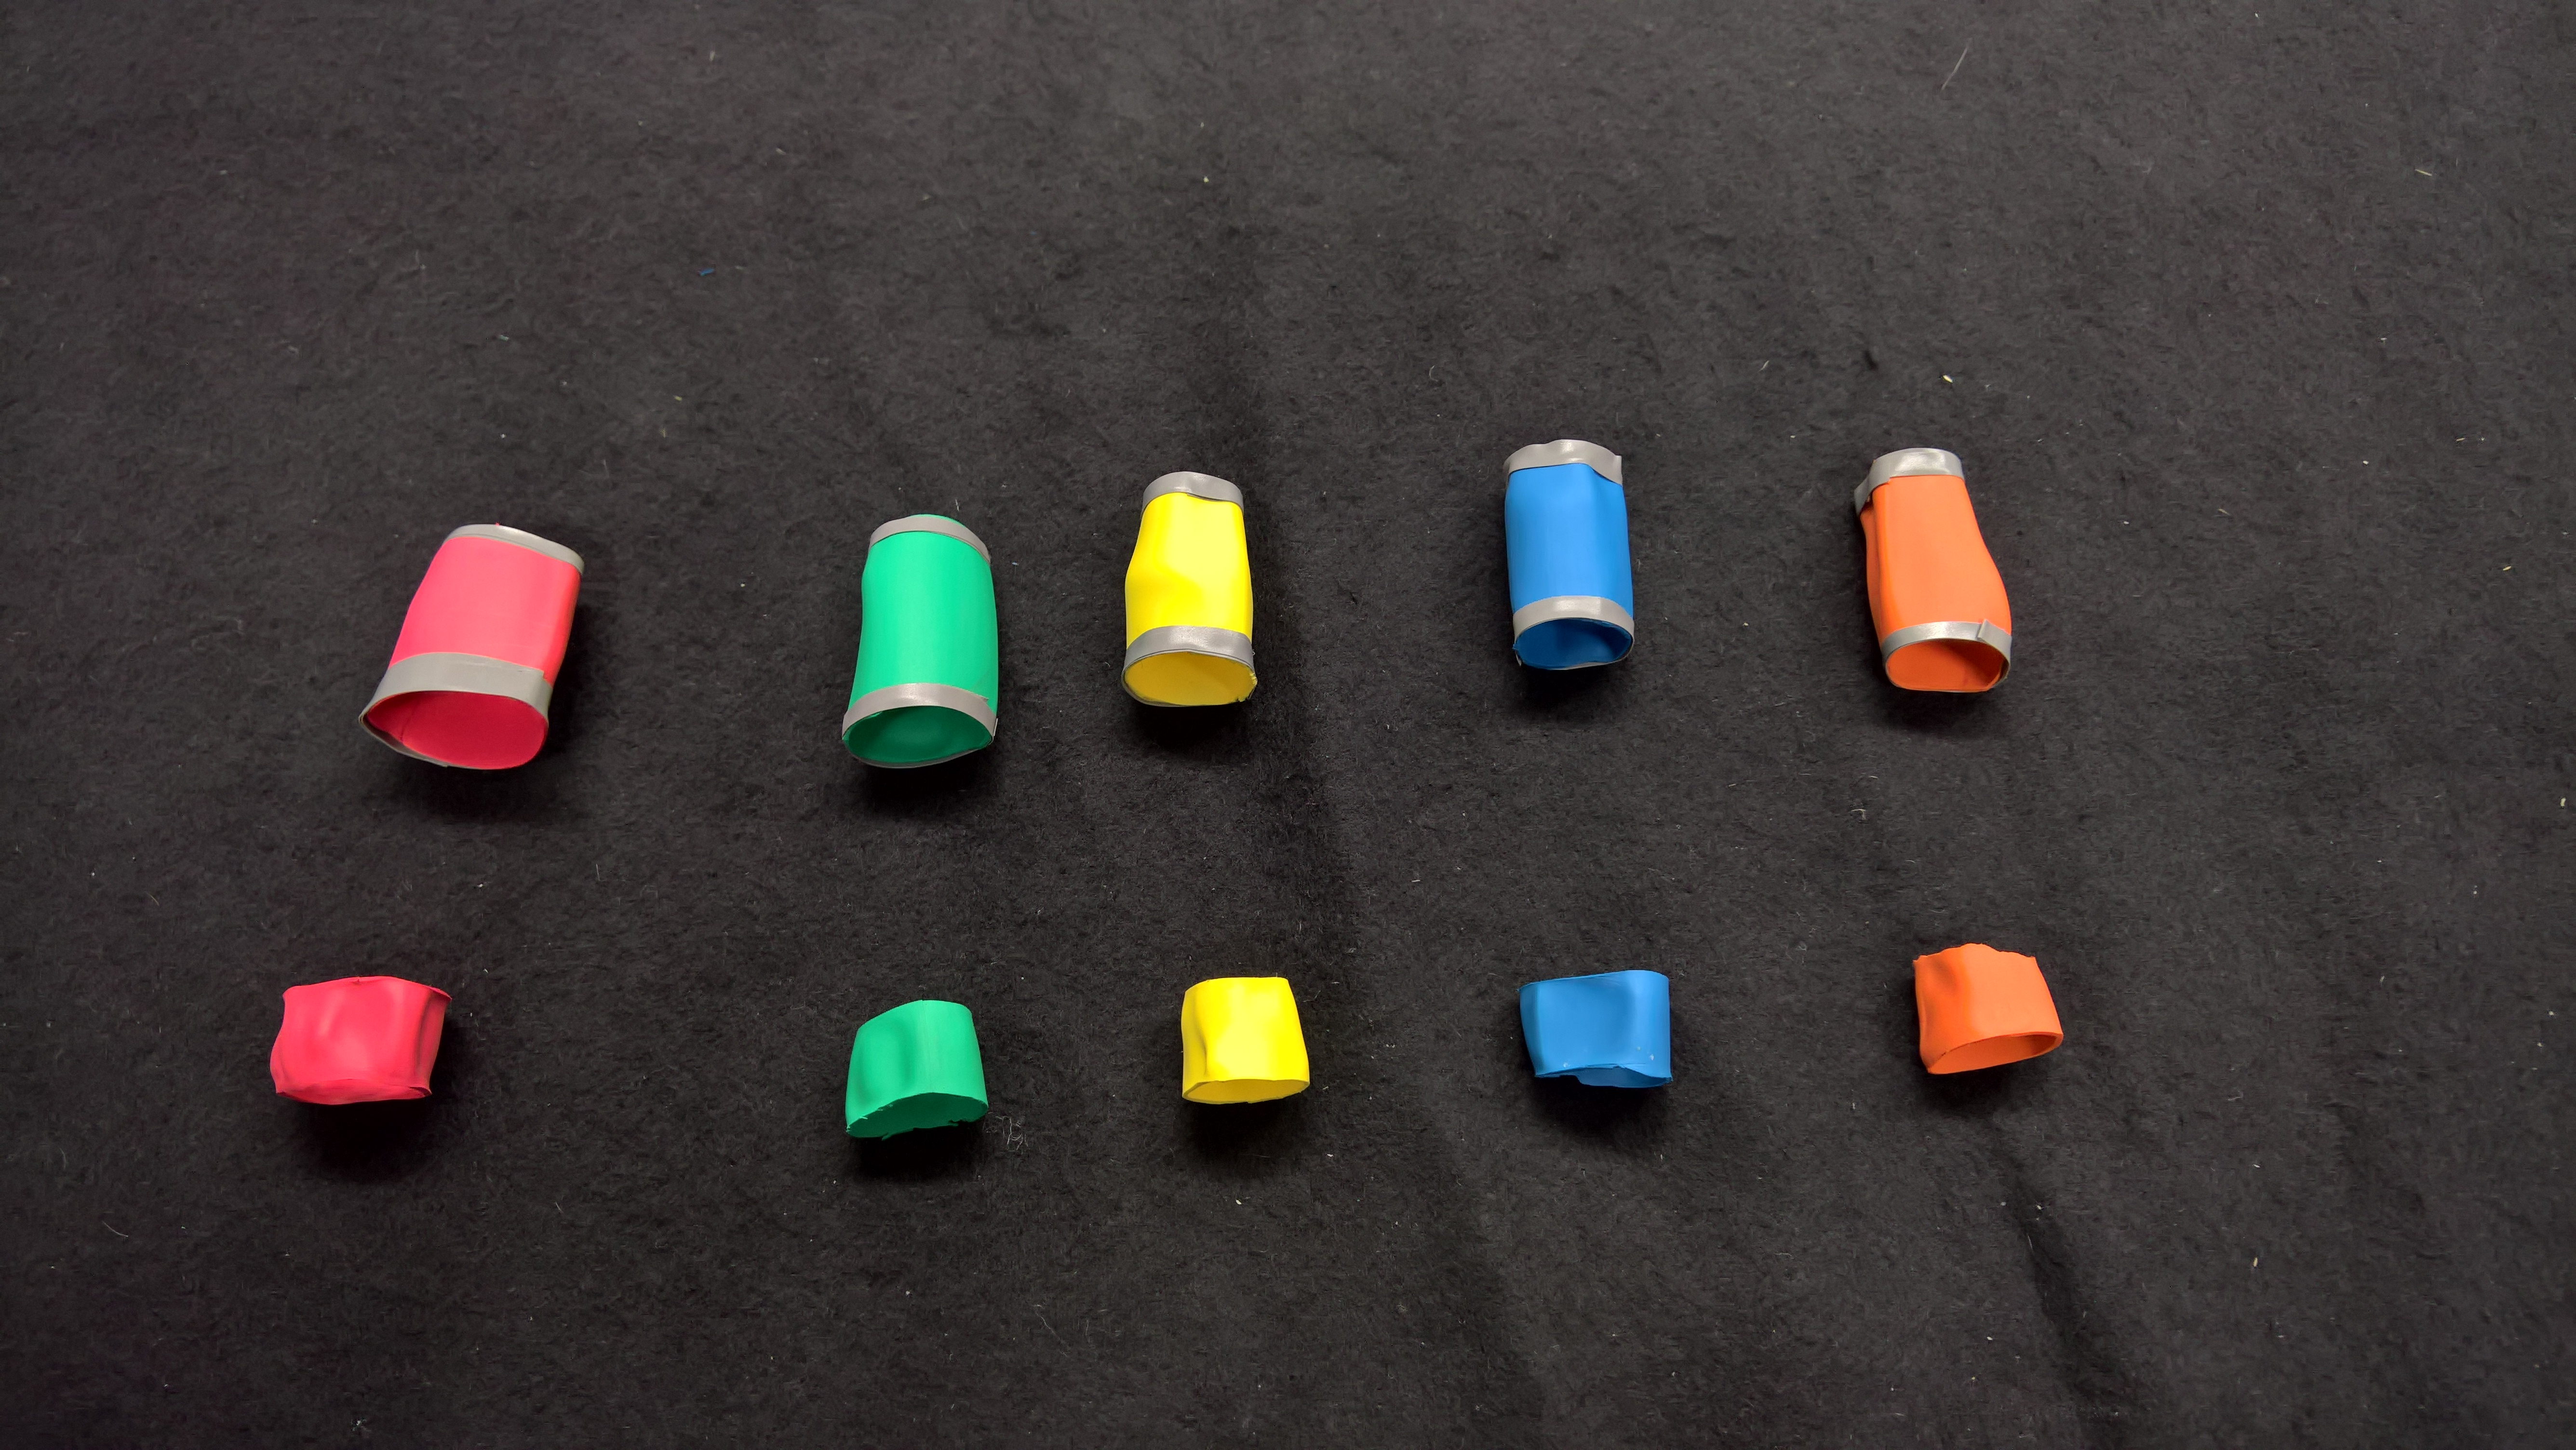
\includegraphics[width=\textwidth/2]{images/small_and_improved_markers.jpg}
\caption{Improved larger and smaller set of shrink tube color markers }
\label{img:second_color_markers}
\end{figure}
The idea behind this solution was to create a fixed border between the color area of the tracker and the color area of the skin tones. The grey color of the border ensures that this area will not be tracked. The usage of black instead of gray would even furthermore ensure this. 
\\Since the threshold algorithm searches for the largest closed color area in the binary threshold image, this border should cause a separation of unwanted skin reflection area and actual tracker color area. The problem that the resulting color marker area might not be the largest area still persists after this improvement, but this case has to be handled separately.
\\Optical results showed that for the colors lying outside of the red to orange color spectrum that skin reflections produce, the artificial border stabilized the color detection.
\\The idea of using shrink tubing as marker material showed to be suitable except in the cases described above. One downside of the material is that the displayed colors are already the highest variety of available colors on the market. Other colors from the green and blue color areas like purple are simply not available or have to be ordered as a special request in larger amounts.
\\Also the original diameter is much larger than a human finger. The used shrink tube is able to be shrunk to one third of its size. The reason for this was to be able to adapt to the varying diameters of the human hand. The shrinking procedure requires a constant amount of heat to be applied to the material to activate the shrinking. The amount of heat that is needed surpasses the heat production of a standard hair dryer since the original application of shrink tubing is on heat resistant cables. The heat that needs to be applied can easily be more than 100 degree Celsius, which makes a direct application on the users hand highly insecure.
\\\\For the prototype, the shrink tube parts were shrunk with a standard cigarette lighter and continuously fitted onto the user finger until the desired form was reached. This method showed to  be sub optimal, since the flame of the lighter produces only a punctual heat source. This caused uneven shrinkage of the heated parts. This can lead to cavities or bumps in the material and change the reflection properties at these points. A regulated heat gun would probably generate better results.
\\To get smoother shrinking results, parts of PVC tubing with the correct diameter could be used as dummy parts for the main part of the shrinking.\\
\\Another approach that was tested was the usage of matte acrylic paint to cover parts or even the whole finger. The matte acrylic paint comes with the benefits of being easily to apply to the finger. Acrylic paint is available in much more color variations than the shrink tube. The finger coating is dry in under a minute after application. Adaption for finger size is automatically included in the application process. If the tracking system does not need to evaluate for hand rotation, i.e. the working principle is a top on view, a nail polish style application of the color on the fingernail can be sufficient for the tracking system. The thumb needs to be treated separately, as it has more rotation capabilities than the other fingers. The thumb should be marked completely on all sides to achieve a constant tracking. If hand orientation is tracked, the other fingers should be completely marked as well.
\todo{replace with image from final acrylic color setup}
\begin{figure}[H]
\centering
\includegraphics[width=\textwidth/2]{images/different_markers.jpg}
\caption{Different types of tested markers. Thumb with complete acrylic coloring, index and ring finger with smaller shrink tube markers, middle finger with nail polish style acrylic color and little finger with large improved marker}
\label{img:differnt_markers}
\end{figure}
The best tracking results in terms of stability and color separation were achieved with the acrylic paint as marker material. For the colors a mixture of blue and green color tones together with red tones in the purple and magenta section were chosen as the final colors.
\todo{Measurements} The usage of the acrylic color also provides the least degradation in terms of gripping haptics on the fingers.
\subsection{Depth measurement accuracy}
To determine the accuracy of the system for it's depth measurement values a simple test bench setup was used. The camera rig was aligned horizontally and fixed to the test bench. A large sized colored marker (75 mm x 50 mm) was used as target for detection. The marker marker was positioned at altering distances from the camera rig along the central axis of the camera rig. The height at which the camera rig is positioned in the experiment setup will be around 100 cm, so the measured distances started at 100 cm from the camera and were decremented in steps of 5 cm until 20 cm in front of the Camera Rig(see Appendix Table \ref{Depth measurement Values} and Figure \ref{char:DisparityToDistanceChart}).
\begin{figure}[H]
\includegraphics[width=\textwidth]{images/Disparity_to_distance.JPG}
\caption{Chart showing the results of the disparity measurement with a plotted trend line}
\label{char:DisparityToDistanceChart} 
\end{figure}The accuracy of the camera system is limited by the number of pixels in relation to the camera view angle:\\
\begin{equation}
\Delta\varphi=\frac{\varphi_0}{x_0}
\end{equation}
\todo{rework text formulation}
With the system set up at 640 pixels of image width and a horizontal viewing angle of $62.5^\circ$, $\Delta\varphi$ is equal to $0.0977\frac{1^\circ}{pixel}$.
The resulting error would be:
\begin{equation}
\frac{\tan \varphi}{\tan(\varphi -\Delta\varphi)}=\frac{\Delta D+D}{D}
\end{equation}
\begin{equation}
\label{equ:delta_d}
\Delta D=\frac{D^{2}}{B} tan(\Delta\varphi)
\end{equation}
The system error for a $D=100cm$ would therefore result in about $2cm$ of possible error.
As the measured values show deviations of up to $5\%$ from the correct value, the function from the trend line displayed in Figure \ref{char:DisparityToDistanceChart} was taken as a correcting factor for the depth calculation.
\\Equation \ref{equ:delta_d} uses the uncorrected values for the calculation. Values lying on the trend lineof Figure \ref{char:DisparityToDistanceChart} should correspond more exactly to the correct distance values \cite{ManafA.Mahammed.2013}. The equation can be rewritten to:
\begin{equation}
\label{equ:power_function}
D=k*x^{z}
\end{equation}
with K being:
\begin{equation}
k=\frac{Bx_0}{2\tan(\frac{\varphi_0}{2}+\phi)}
\end{equation}
and x the disparity in pixels.
The $\phi$ term in the equation above is used as a compensation for possible alignment errors.
The trend line, which is fit to the measurements in Figure \ref{char:DisparityToDistanceChart} represents the the function needed to fulfill Equation \ref{equ:power_function}.The calculated values are $k=4543.3$ and $z=-1.035$.
With the utilization of the corrected value formula, the accuracy of the depth measurement results is acceptable for the prototype application. For future work, the distance measurement procedure could be applied with more measurement points to refine the resulting function for more precision. The measurement values that were retrieved can be found in the Appendix Table \ref{Depth measurement Values}.
\section{Inverse kinematics algorithm}
- missing feature for parabolic constraint curves
- measure calculation times 
- setup difficulty
\begin{figure}[H]
\centering
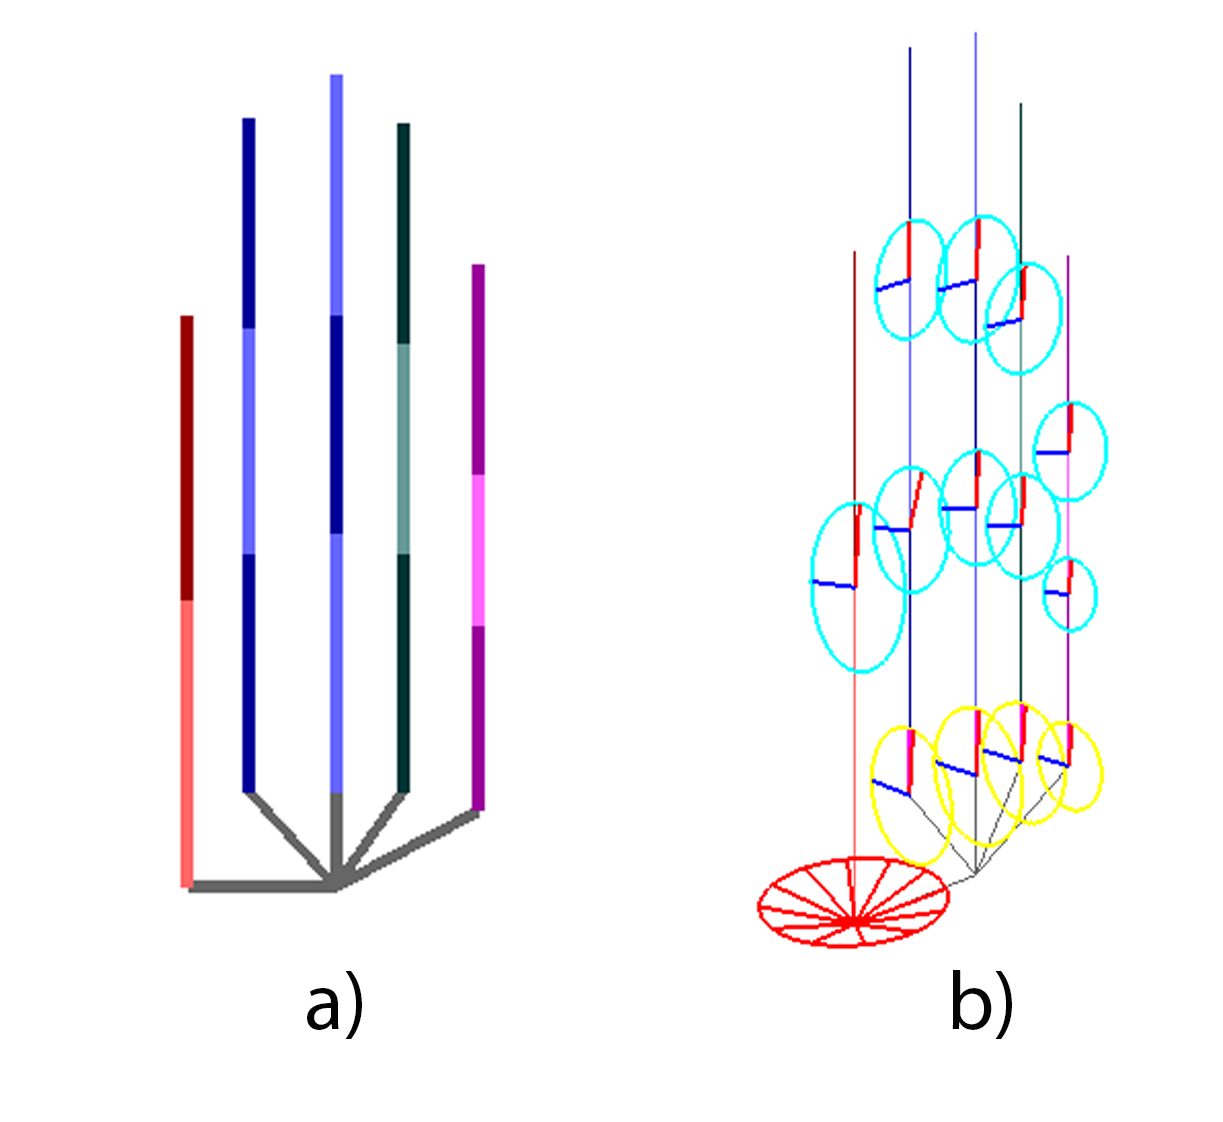
\includegraphics[width=\textwidth/2]{images/hand_model_combo.png}
\caption{Hand model representatio of the used IK Framework: a) Kinematic chains and base structure, b) hand model with visualized movement constraints}
\label{img:netzwerk_diagram} 
\end{figure}

